\documentclass[xcolor=dvipsnames]{beamer}

\usetheme{Berkeley}

\setbeamertemplate{footline}[frame number]


\usepackage{inputenc}
\usepackage{amsmath}
\usepackage{graphicx}
\usepackage{hyperref}

\title{Theory and Algorithm for Generalized Memory Partitioning in High-Level Synthesis}
\subtitle{Yuxin W., Peng L., Jason C.}

\author{FPGA'14, Feb 26-28, 2014}

\begin{document}
    
    \begin{frame}

        \maketitle

        \begin{center}
            Presented by: Akshay G
        \end{center}

    \end{frame}

    \begin{frame}{About the Authors}

        \begin{figure}
            
\includegraphics[scale=0.6]{CECA.PNG}
        \end{figure}

        \begin{figure}
            
\includegraphics[scale=0.6]{PKU-UCLA.PNG}
        \end{figure}
        
    \end{frame}

    \begin{frame}{Outline}

        \begin{itemize}
            \item Introduction. 
            \item Background. 
            \item Bank Partitioning.
            \item Intra-bank Offset.
            \item Results. 
            \item Comments. 
        \end{itemize}
        
    \end{frame}

    \section{Introduction}
    \begin{frame}{Introduction}

        \begin{itemize}
            \item Memory Partitioning problem.
            \item Partitioning given multiple memory ports?
            \item Algorithm parametric to partition scheme?
            \item Modular to memory ports?
        \end{itemize}
        
    \end{frame}

    \begin{frame}{Memory Partitioning}

        \begin{figure}
            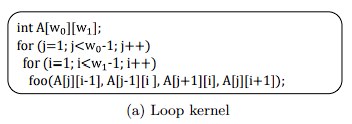
\includegraphics{LoopExample.PNG}
        \end{figure}

        \begin{figure}
            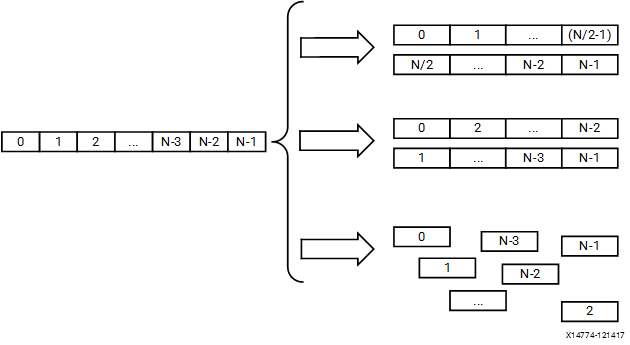
\includegraphics[scale=0.6]{MemPaart.png}
        \end{figure}
        
    \end{frame}

    \begin{frame}{Partitioning Schemes}

        \begin{figure}
            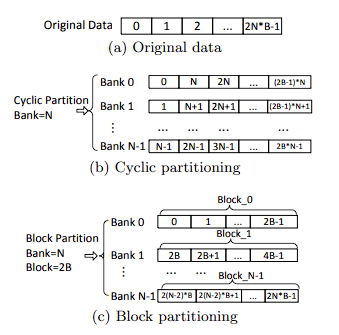
\includegraphics{PartSchemes.PNG}
        \end{figure}
        
    \end{frame}

    \begin{frame}{Efficient Mapping}

        \begin{figure}
            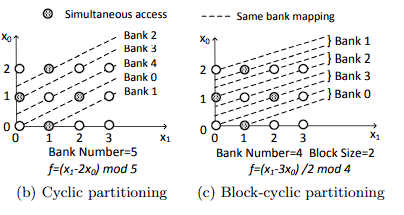
\includegraphics{CyclevsHybrid.PNG}
        \end{figure}
        
    \end{frame}

    \section{Background}
    \begin{frame}{Towards Theory: Symbols!!}

        \begin{figure}
            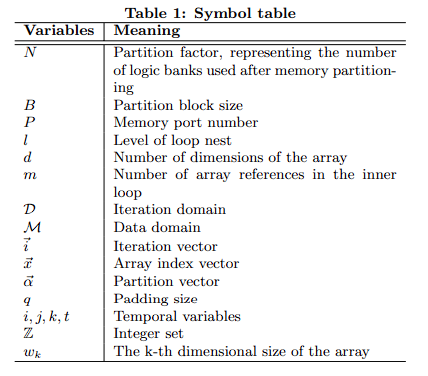
\includegraphics[scale=0.8]{MathSymb.PNG}
        \end{figure}
        
    \end{frame}

    \begin{frame}{Iteration Vector and Affine Reference}

        \begin{figure}
            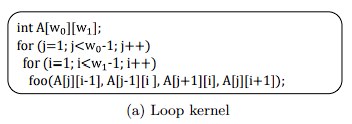
\includegraphics{LoopExample.PNG}
        \end{figure}

        \begin{figure}
            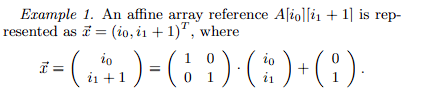
\includegraphics{AffineRef.PNG}
        \end{figure}
        
    \end{frame}

    \begin{frame}{Framing the Partitioning Problem}

        Two parts:
        \begin{itemize}
            \item Bank Minimization.
            \item Storage Minimization.
        \end{itemize} 

        \begin{columns}
            
            \begin{column}{0.5\textwidth}

                \begin{figure}
                    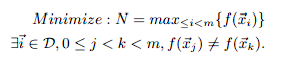
\includegraphics[scale=0.8]{BankPart.PNG}
                \end{figure}
                
            \end{column}

            \begin{column}{0.5\textwidth}

                \begin{figure}
                    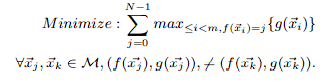
\includegraphics[scale=0.8]{StorePart.PNG}
                \end{figure}
                
            \end{column}

        \end{columns}
        
    \end{frame}

    \section{Bank Partitioning}
    \begin{frame}{Bank Mapping}

        \begin{figure}
            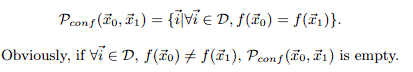
\includegraphics{BankMap.PNG}
        \end{figure}

        \begin{figure}
            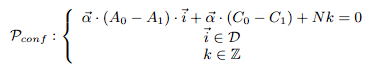
\includegraphics{BankMapCyclic.PNG}
        \end{figure}
        
    \end{frame}

    \begin{frame}{Bank Mapping: Multi Port}

        \begin{figure}
            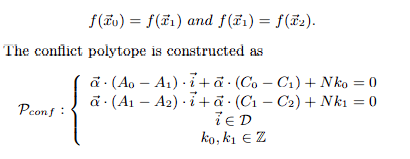
\includegraphics{MultiPortExtn.PNG}
        \end{figure}
        
    \end{frame}

    \section{Intra-bank Offset}
    \begin{frame}{Intra-bank Offset Mapping}

        \begin{figure}
            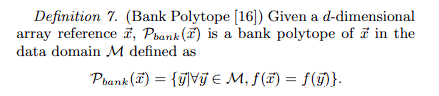
\includegraphics{BankPoly.PNG}
        \end{figure}

        \begin{figure}
            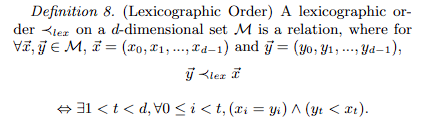
\includegraphics{LexOrder.PNG}
        \end{figure}
        
    \end{frame}

    \begin{frame}{Offset Mapping Intuition}

        \begin{figure}
            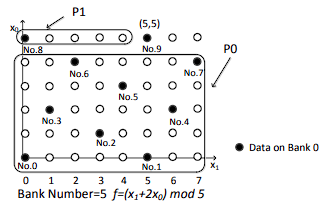
\includegraphics{BankMapIntuition.PNG}
        \end{figure}

        \begin{figure}
            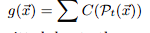
\includegraphics{OffsetEq.PNG}
        \end{figure}
        
    \end{frame}

    \section{Results}
    \begin{frame}{Algorithm Flow}

        \begin{figure}
            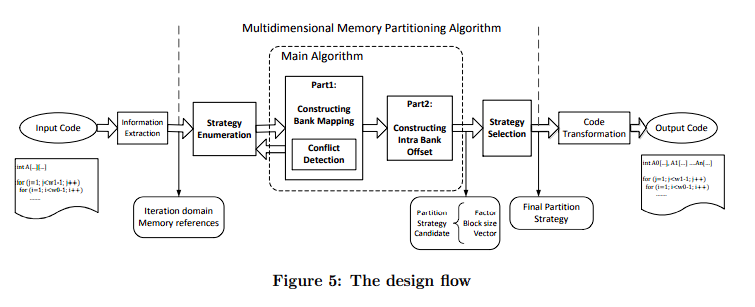
\includegraphics[scale=0.6]{FinalPipeline.PNG}
        \end{figure}
        
    \end{frame}

    \begin{frame}{Results (compared to previous work LTB)}

        \begin{figure}
            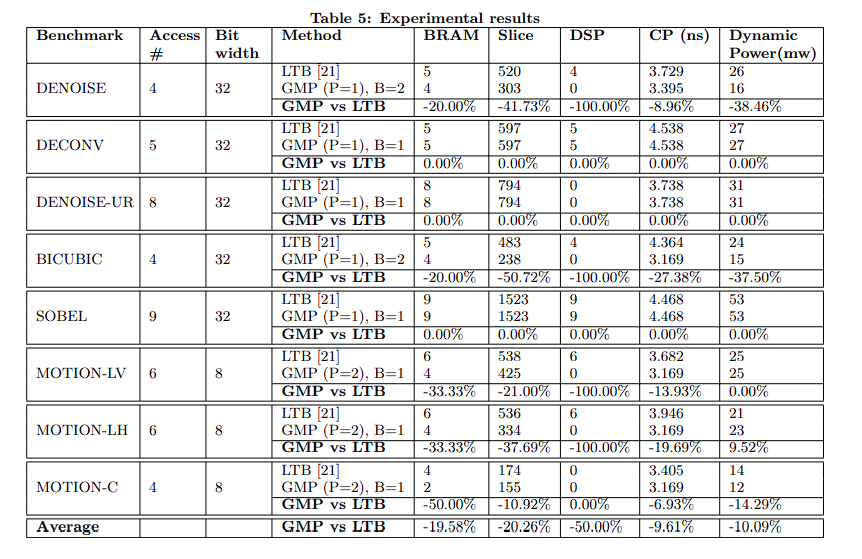
\includegraphics[scale=0.6]{Experiment.PNG}
        \end{figure}
        
    \end{frame}

    \section{Comments}
    \begin{frame}{Limitations?}

        \begin{itemize}
            \item Experiments on Partitioning algorithm performance.
            \item Lack of some important mathematical details (some function definitions missing). 
        \end{itemize}
        
    \end{frame}

    \begin{frame}{Thank you}

        Questions?
        
    \end{frame}

\end{document}